\documentclass[12pt,peerreviewca, a4paper, onecolumn]{article}

\pagenumbering{gobble}

\title{\LARGE\textbf{Looking For Caresses with MiRo}\\\large For Social Robotics Course 2018/19}
\author{\large{Torielli Davide \quad Fusaro Fabio} \\
	\small EMARO - European Master on Advanced Robotics\\
	\small DIBRIS - Dip. Informatica, Bioingegneria, Robotica, Ing. Dei Sistemi\\
	\small Universit\`{a} Degli Studi Di Genova, \today}

\usepackage{hyperref}
\hypersetup{colorlinks=true, linkcolor=blue, urlcolor = blue}
\usepackage[a4paper,left=40px,right=40px,top=50px,bottom=10px,
includefoot,heightrounded]{geometry}
\usepackage{amsmath}
\usepackage{relsize}
\usepackage{amssymb}
\usepackage{graphicx}
\graphicspath{ {./images/} }
\usepackage{caption}
\usepackage{floatrow}
\usepackage{titlesec}
\titleformat{\section}[block]{\large\bfseries}{\thesection}{4mm}{}

\titleformat{\subsection}[block]{\normalsize\bfseries}{\thesubsection}{2mm}{}

\begin{document}
	\maketitle
	
	\section{Introduction}
	MiRo (from \href{http://consequentialrobotics.com/}{Consequential Robotics}) is a flexible platform suited for developing companion robots. It has different sensors to interact with the environment: cameras, cliff sensors, light sensor, sonar, microphone.\\
	In this project, MiRo behave as companion pet, standing on the desk while the user is working (for example, at pc). We exploit joints and sensors to make the robot interact with the user, and make MiRo act like a pet should do: make noise, show sleepiness, wag tail if happy, and so on. Like a real pet, MiRo wants attentions from the user.\\ 
	We use a \textbf{loneliness} value which ranges from 0 to 100. When it is high, MiRo will more probably look for caresses, because it feels lonely. While the interaction is going on (i.e., the user caresses  MiRo), this value goes down. The more the level is low, the more MiRo will probably return to sleep.
	
	\section{The Code}
	\begin{center}
		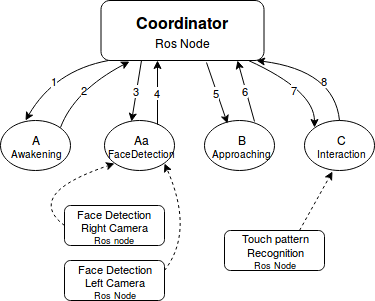
\includegraphics[scale=0.5]{diagram}
	\end{center}
	{\small The diagram on the code structure: straight lines with numbers resprent execution flow. After step 8 the cycle begins again from step 1. Dotted lines represent data exchanged through ROS publish-subscribe method. The communications with the robot (again with ROS topics), to receive sensor data and send platform commands, are not shown.}\\

	\noindent The \textbf{coordinator} is a ROS node responsible to handle different classes related to the 4 different phases: Awakening (\ref{subsec:a}); Face Recognition (\ref{subsec:aa}); Approaching (\ref{subsec:b}); Interaction (\ref{subsec:c}).
	\subsection{Task A: Awakening Phase}
	\label{subsec:a}
	In task A, MiRo is sleeping. The task sends through ROS topic commands to show this (closed eyelids and head down). While sleeping, \textbf{loneliness} value increases, until MiRo wakes up alone or until he is touched by the user.
	\subsection{Task Aa: Face Recognition Phase}	\label{subsec:aa}
	In task Aa MiRo looks for the user face. To do this, we rely on the \textit{face detector} node  (from \href{http://wiki.ros.org/opencv_apps}{opencv\_apps} package). This node is subscribed to the topic where left and right cameras publish the image flow, and publish face detection infos on another topic. We read from this last topic if a face is detected or not.
	If MiRo does not see a face with neither cameras, it turns on z axis. If he sees a face with only one camera, it turns a bit slower clockwise or counter-clockwise to catch the face with both cameras, and at this point it stops turning. When MiRo sees the face with both cameras for 1.5 consecutively seconds, the task finishes.
	\subsection{Task B: Approaching Phase}	\label{subsec:b}
	MiRo gets near to the user using the sonar on his muzzle. The user should put the hand toward MiRo's muzzle, to start interaction with him. If the sonar detects something (i.e., the hand) sufficently near, MiRo stops and next phase starts.
	\subsection{Task C: Interaction Phase} 	\label{subsec:c} 
	The user can choose to interact or not with MiRo. If he rubs him on the body, the \textbf{loneliness} value will decrease. Meanwhile, MiRo will act like real pet: the more he is rubbed the more he showns his happiness wagging the tail, moving the ears, and making ``mammal'' sounds.\\
	If the user does not want to interact any more, he must pat MiRo on head, and he will immediately go to sleep, but with a higher value of \textbf{loneliness}.\\
	To understand the touches, we use a node implemented by \href{https://github.com/EmaroLab/Miro_SocialRobot/blob/master/README.md}{others}.
	The chance to make MiRo go to sleep increases if \textbf{loneliness} value decreases. After the interaction phase, the awakening phase is recalled and the cycle repeats. 
	
	\section{Further Works}
	\subsection{Experiment}
	Feedback from different people would be useful to improve the behaviour of MiRo and to make him acting even more as a real pet.\\
	Settings for the experiment could be:
	\begin{itemize}
		\item Take different MiRo behaviours in a certain situation (e.g. interaction phase).
		\vspace{-6px}
		\item Find an heterogeneous group of people (e.g. male and female, young and old) as experimental units.
		\vspace{-6px}
		\item Assign the different MiRo behaviours to all experimental units, i.e. \textit{within-subject} assign method.
		\vspace{-18px}
		\item Define the variables to be measured: e.g. given the MiRo sensors, how people act to send away him in the interaction phase.
		\vspace{-6px}
		\item Define well the measure: a questionnaire is needed in order to understand how much the MiRo behaviours are similar to a real pet. A Likert scale type may be used. Also, a pre-questionnaire can be done in order to understand the attitude of each person toward a companion pet robot.
		\vspace{-6px}
		\item Analyse results and use them to improve MiRo general behaviour.
	\end{itemize}
	
	
	
	\subsection{Code improvements}
	The more critical phase is the interaction one. The sensors of MiRo are really simple (binary ones) and the ones on the head are not so intuitive and easy to use. Also, they are positioned on particular points, and not spread on the whole body. For this, any pattern recognition algorithm is difficult to use. So to solve the problem we differentiate the behaviour basing on body and head touches. If the user wants to interact with MiRo, he has to rub him on body, and, if not, he has to touch him on the head. This is done to avoid confusion in detecting the pattern. A further work can focuses on this particular problem.\\
	Also the face recognition can be improved helping in some way the task; for example, moving and not only turning the body or exploiting the other joints of the neck (pitch and yaw).\\
	Another work could be done towards improving the interaction, making use, for example, also of the microphones on MiRo ears.
 
	 
		

	
\end{document}